\documentclass{report}

\usepackage{amsmath}
\usepackage{graphicx}


\begin{document}
\chapter*{Oblique Spherical Triangles Toolbox}
\section*{Introduction}

Spherical trigonometry is generally much more involved than its
plain counterpart. A nice example of this is the seemingly simple
spherical triangle (a triangle on a sphere). The usual laws for
plain triangles no longer hold: the sum of the angles can easily
exceed 180$^\circ$, the Pythagorean theorem does not apply when
one of the angles is 90$^\circ$, and so on.

The formulas to find quantities in spherical triangles are quite
tedious. Their derivation is also not very trivial, which makes
them also harder to remember. For that reason, this little toolbox
has been created.

\begin{figure}[h!]
         \centering
         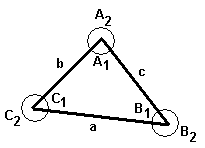
\includegraphics[bb=0 0 205 148]{OblSphTri.png}
         \caption{An arbitrary oblique spherical triangle.}
         \label{fig}
\end{figure}

A general spherical triangle is shown in Figure \ref{fig}. Note
that there are two angles associated with every ``corner'' of the
triangle. Also keep in mind that each ``side'' of a spherical
triangle is not a length, but an angle (with respect to the center
of the sphere). Then, if 3 arbitrary quantities (angles, sides)
are given and the other 3 quantities are to be found, 6 different
sub-problems can be identified. These can be defined as
follows:

\begin{table}[h!]
  \centering
  \caption{The 6 categories of oblique spherical triangles.
  Adapted from Table~A-1 in~\cite{Wertz2001}}
  \label{table}
  \begin{tabular}{|c||c|c|c|}\hline
         \textbf{Type}   & \textbf{Given} & \textbf{Find} &
         \textbf{No. of Solutions}\\\hline
         Side-Side-Side  & a, b, c & A, B, C & 0 or 2\\
         Side-Side-Angle & a, b, A & B, C, c & 0 or 2\\
         Side-Angle-Side & a, C, b & A, B, c & 2\\
         Angle-Angle-Side & A, B, a & b, c, C & 0 or 2\\
         Angle-Side-Angle & A, c, B & a, C, b & 2\\
         Angle-Angle-Angle & A, B, C & a, b, c & 0 or 2\\\hline
  \end{tabular}
\end{table}

All these problems involve rather long equations which will not be
repeated here. The interested reader is referred to Appendix A of
\cite{Wertz2001}, or similar standard works on spherical
trigonometry.

\cite{Wertz2001} uses a somewhat unconventional method to automate
solving these problems, namely the \texttt{acos2}-function. Indeed
it is the four-quadrant arccosine function, which is defined as

\[
        \text{acos2}(x) = H(x)\cdot \text{acos}(x),
\]

where $H(x) = +1$ if $x < 180^\circ$, and $H(x) = -1$ if $x >
180^\circ$. Defined like this, the \texttt{acos2} function
completely does away with the need of user intervention when
solving either of the 6 sub-problems, thus enabling full
automation.

\section*{The Toolbox}
This little toolbox is simply an implementation of all of the
above sub-problems. All functions are fully vectorized and should
work for vector or matrix input. The main components are:

\subsubsection{\texttt{sss.m} and \texttt{sssd.m}}
Usage:

\[
         \texttt{[A1, B1, C1, A2, B2, C2] = sss(a, b, c)}
\]

Returns both solutions to the Side-Side-Side problem. If no
solution exists, \texttt{NaN} is returned. Uses the \texttt{acos2}
function. \texttt{sss.m} uses radians, whereas \texttt{sssd.m}
uses degrees.

\subsubsection{\texttt{ssa.m} and \texttt{ssad.m}}
Usage:

\[
         \texttt{[B1, C1, c1, B2, C2, c2] = ssa(a, b, A)}
\]

Returns both solutions to the Side-Side-Angle problem. If no
solution exists, \texttt{NaN} is returned. Uses the
implementations of the Middle Angle Law (\texttt{mal.m}) and
Middle Side Law (\texttt{msl.m}). \texttt{ssa.m} uses radians,
whereas \texttt{ssad.m} uses degrees.

\subsubsection{\texttt{sas.m} and \texttt{sasd.m}}
Usage:

\[
         \texttt{[c1, A1, B1, c2, A2, B2] = sas(a, C, b)}
\]

Returns both solutions to the Side-Angle-Side problem. Uses the
\texttt{acos2} function. \texttt{sas.m} uses radians, whereas
\texttt{sasd.m} uses degrees.

\subsubsection{\texttt{aas.m} and \texttt{aasd.m}}
Usage:

\[
         \texttt{[b1, c1, C1, b2, c2, C2] = aas(A, B, a)}
\]

Returns both solutions to the Angle-Angle-Side problem. If no
solution exists, \texttt{NaN} is returned. Uses the
implementations of the Middle Angle Law (\texttt{mal.m}) and
Middle Side Law (\texttt{msl.m}). \texttt{aas.m} uses radians,
whereas \texttt{aasd.m} uses degrees.

\subsubsection{\texttt{asa.m} and \texttt{asad.m}}
Usage:

\[
         \texttt{[C1, a1, b1, C2, a2, b2] = asa(A, B, c)}
\]

Returns both solutions to the Angle-Side-Angle problem. Uses the
\texttt{acos2} function. \texttt{asa.m} uses radians, whereas
\texttt{asad.m} uses degrees.

\subsubsection{\texttt{aaa.m} and \texttt{aaad.m}}
Usage:

\[
         \texttt{[a1, b1, c1, a2, b2, c2] = aaa(A, B, C)}
\]

Returns both solutions to the Angle-Angle-Angle problem. If no
solution exists, \texttt{NaN} is returned. Uses the \texttt{acos2}
function. \texttt{aaa.m} uses radians, whereas \texttt{aaad.m}
uses degrees.

\section*{Auxiliary Functions}
These are included in the auxiliary folder. They are:

\subsubsection{\texttt{mal.m} and \texttt{mald.m}}
The implementation of the Middle-Angle Law for spherical
triangles:

\begin{eqnarray*}
\sin c &=& \frac{\sin a\cos b\cos B + \sin b \cos a \cos A}
{1-\sin a \sin b \sin A \sin B},\\
\cos c &=& \frac{\cos a\cos b + \sin a \sin b \cos A\cos B}
{1-\sin a \sin b \sin A \sin B},\\
c &=& \text{atan2}(\sin c,\,\cos c).
\end{eqnarray*}

This function is used only internally. Instructions on how to use
it manually are given in the help.

\subsubsection{\texttt{msl.m} and \texttt{msld.m}}
The implementation of the Middle-Side Law for spherical triangles:

\begin{eqnarray*}
\sin C &=& \frac{\sin A\cos B\cos b + \sin B \cos A \cos a}
{1-\sin a \sin b \sin A \sin B},\\
\cos C &=& \frac{-\cos A\cos B + \sin A \sin B \cos a\cos b}
{1-\sin a \sin b \sin A \sin B},\\
c &=& \text{atan2}(\sin c,\,\cos c).
\end{eqnarray*}

This function is used only internally. Instructions on how to use
it manually are given in the help.

\subsubsection{\texttt{acos2.m}, \texttt{acos2d.m}, \texttt{H.m} and \texttt{Hd.m}}
\texttt{H.m} and \texttt{Hd.m} are the implementations of the
Hemisphere-function $H(x)$, which determines the sign of the
arccosine in \texttt{acos2.m} or \texttt{acos2d.m}.

This function is used only internally. Instructions on how to use
it manually are given in the help.

\subsubsection{\texttt{blkassign.m}}
This is a tool that prevents long blocks of assignments, when each
variable to be assigned is a column or row of a given matrix.
Normally, this is done as

\begin{eqnarray*}
    A &=& \texttt{rand}(5);\\
    a &=& A(:,\,1);\\
    b &=& A(:,\,2);\\
    c &=& A(:,\,3);\\
    &&\text{etc.}
\end{eqnarray*}

but with \texttt{blkassign.m}, this can be shortened as

\begin{eqnarray*}
    A &=& \texttt{rand}(5);\\
    \left[a,\,b,\,c,\,\dots\right] &=& \texttt{blkassign}(A);\\
\end{eqnarray*}

Also this function is used internally only. Instructions on how to
use it manually are given in the help.

\bibliographystyle{plainnat}
\bibliography{bibliography}
\end{document}
